%% LyX 2.1.4 created this file.  For more info, see http://www.lyx.org/.
%% Do not edit unless you really know what you are doing.
\documentclass[a4paper,twoside,czech,czech,cleardoublepage=empty,BCOR15mm,DIV12]{scrreprt}
\usepackage{tgtermes}
\usepackage{tgheros}
\usepackage{tgcursor}
\usepackage{newtxmath}
\usepackage[T1]{fontenc}
\usepackage[utf8]{inputenc}
\usepackage{babel}
\usepackage{float}
\usepackage{url}
\usepackage{graphicx}
\usepackage[unicode=true,pdfusetitle,
 bookmarks=true,bookmarksnumbered=false,bookmarksopen=false,
 breaklinks=false,pdfborder={0 0 1},backref=false,colorlinks=false]
 {hyperref}

\makeatletter

%%%%%%%%%%%%%%%%%%%%%%%%%%%%%% LyX specific LaTeX commands.
\pdfpageheight\paperheight
\pdfpagewidth\paperwidth

\newcommand{\noun}[1]{\textsc{#1}}
\floatstyle{ruled}
\newfloat{algorithm}{tbp}{loa}[chapter]
\providecommand{\algorithmname}{Algoritmus}
\floatname{algorithm}{\protect\algorithmname}

%%%%%%%%%%%%%%%%%%%%%%%%%%%%%% Textclass specific LaTeX commands.
\newenvironment{lyxcode}
{\par\begin{list}{}{
\setlength{\rightmargin}{\leftmargin}
\setlength{\listparindent}{0pt}% needed for AMS classes
\raggedright
\setlength{\itemsep}{0pt}
\setlength{\parsep}{0pt}
\normalfont\ttfamily}%
 \item[]}
{\end{list}}

%%%%%%%%%%%%%%%%%%%%%%%%%%%%%% User specified LaTeX commands.
%<-------------------------------společná nastavení------------------------------>
\usepackage[numbers,sort&compress]{natbib} %balíček pro citace literatury  
\usepackage{algorithmic}
\usepackage{color}%kvůli barvám ČVUT
\newcommand{\BibTeX}{{\sc Bib}\TeX}%BibTeX logo
\usepackage{multicol}




%<-----------------------------volání stylů----------------------------------------->
% (znak % je označení komentáře: co je za ním, není aktivní)

%<--------matematické písmo--------------------------------------->

%\usepackage[helvet]{packages/sfmath}%matematika ala helvetica



%<------------------------------záhlaví stránek------------------------------------>
%\usepackage{packages/bc-headings}
\usepackage{packages/bc-fancyhdr}

%<------------------------------hlavičky kapitol------------------------------------>
%\usepackage{packages/bc-neueskapitel}
\usepackage{packages/bc-fancychap}

\makeatother

\begin{document}
~\thispagestyle{empty}{\small{}~\vfill{}
}{\small \par}

\noindent {\small{}Na tomto místě mohou být napsána případná poděkování
(vedoucímu práce, konzultantovi, tomu kdo půjčil software, literaturu,
poskytl data apod.). \newpage{}}{\small \par}

~\thispagestyle{empty}\vfill{}
Tato stránka je tzv. protititul a je graficky součástí titulní stránky.
Nechte ji prázdnou, nebo na ni umístěte vhodnou fotografii či ilustraci.

\cleardoublepage{}~\thispagestyle{empty}\begin{center}\pagenumbering{roman}\vspace{10mm}


\textsf{\textsc{\noun{\LARGE{}České vysoké učení technické v Praze}}}\\
\vspace{0.5em}
\textsf{\textsc{\noun{\LARGE{}Fakulta elektrotechnická}}}\\
\vspace*{1em}
\textsf{\textsc{\noun{\Large{}katedra kybernetiky}}}\vspace{15mm}


%%% Aby vložení loga  správně fungovalo, je třeba mít soubor lev.png nahraný v pracovním adresáři,
%%% tj. v adresáři, kde se nachází překládaný zdrojový soubor. 

\includegraphics[width=0.3\textwidth]{obrazky/lev}\vspace{15mm}


\textsf{\huge{}BAKALÁŘSKÁ/DIPLOMOVÁ PRÁCE}{\huge \par}

\vspace{15mm}


\textsf{\LARGE{}Název práce}{\LARGE \par}

\vspace{10mm}


\end{center} 

\vspace*{\fill}


\vspace{10mm}

\begin{description}
\item [{{\large{}Autor:}}] \noindent \textsf{\large{}Matěj Račinský}{\large \par}
\item [{{\large{}Vedoucí~práce:}}] \noindent \textsf{\large{}Dr. Martin
Saska}{\large{}\hfill{}}\textsf{\large{}Praha,}{\large{} \the\year % nebo doplňte rok vzniku vaší bakalářské práce
}{\large \par}
\end{description}
\clearpage{}

{\small{}\thispagestyle{plain}\addcontentsline{toc}{chapter}{Abstrakt} }{\small \par}

\noindent {\small{}~\vfill{}
}{\small \par}
\begin{description}
\item [{{\small{}Název~práce:}}] \noindent {\small{}Název bakalářské práce}{\small \par}
\item [{{\small{}Autor:}}] \noindent {\small{}Matěj Račinský}{\small \par}
\item [{{\small{}Katedra~(ústav):}}] \noindent Kate{\small{}dra kybernetiky}{\small \par}
\item [{{\small{}Vedoucí~bakalářské~práce:}}] \noindent Dr. Martin Saska
\item [{{\small{}e-mail~vedoucího:}}] \noindent {\small{}saska@labe.felk.cvut.cz}\\
{\small \par}
\item [{{\small{}Abstrakt}}] \noindent {\small{}V předložené práci studujeme...
Uvede se abstrakt v rozsahu 80 až 200 slov. Lorem ipsum dolor sit
amet, consectetuer adipiscing elit. Ut sit amet sem. Mauris nec turpis
ac sem mollis pretium. Suspendisse neque massa, suscipit id, dictum
in, porta at, quam. Nunc suscipit, pede vel elementum pretium, nisl
urna sodales velit, sit amet auctor elit quam id tellus. Nullam sollicitudin.}{\small \par}
\item [{{\small{}Klíčová~slova:}}] \noindent {\small{}klíčová slova (3
až 5)}\\
{\small \par}
\item [{\rule[0.5ex]{1\linewidth}{1pt}}]~{\small \par}
\item [{{\small{}Title:}}] \noindent {\small{}Název bakalářské práce v
angličtině}{\small \par}
\item [{{\small{}Author:}}] \noindent {\small{}Matěj Račinský}{\small \par}
\item [{{\small{}Department:}}] \noindent {\small{}Department of Cybernetics}{\small \par}
\item [{{\small{}Supervisor:}}] \noindent Dr. Martin Saska
\item [{{\small{}Supervisor's~e-mail~address:}}] \noindent {\small{}saska@labe.felk.cvut.cz}\\
{\small \par}
\item [{{\small{}Abstract}}] \noindent {\small{}In the present work we
study ... Uvede se anglický abstrakt v rozsahu 80 až 200 slov. Lorem
ipsum dolor sit amet, consectetuer adipiscing elit. Ut sit amet sem.
Mauris nec turpis ac sem mollis pretium. Suspendisse neque massa,
suscipit id, dictum in, porta at, quam. Nunc suscipit, pede vel elementum
pretium, nisl urna sodales velit, sit amet auctor elit quam id tellus.
Nullam sollicitudin. Donec hendrerit. Aliquam ac nibh. Vivamus mi.
Sed felis. Proin pretium elit in neque. Pellentesque at turpis. Maecenas
convallis. Vestibulum id lectus. }{\small \par}
\item [{{\small{}Keywords:}}] \noindent {\small{}klíčová slova (3 až 5)
v angličtině}{\small \par}
\end{description}
\cleardoublepage{}\thispagestyle{empty}~{\small{}\addcontentsline{toc}{chapter}{Zadání
práce} }{\small \par}



\newpage{}\thispagestyle{empty}~



\newpage{}\thispagestyle{plain}

{\small{}%\setcounter{page}{3} % nastavení číslování stránek
\ }{\small \par}

\noindent {\small{}\vfill{}
 % nastavuje dynamické umístění následujícího textu do spodní části stránky
~}{\small \par}

\noindent {\small{}Prohlašuji, že jsem svou bakalářskou práci napsal(a)
samostatně a výhradně s použitím citovaných pramenů. Souhlasím se
zapůjčováním práce a jejím zveřejňováním.}{\small \par}

{\small{}\bigskip{}
}\noindent {\small{} V Praze dne \today\hspace{\fill}Jméno Příjmení
+ podpis}\\
{\small{} % doplňte patřičné datum, jméno a příjmení
}{\small \par}

{\small{}%%%   Výtisk pak na tomto míste nezapomeňte PODEPSAT!
%%%                                         *********
}{\small \par}

\cleardoublepage{}

\thispagestyle{empty}{\small{}\tableofcontents{}% vkládá automaticky generovaný obsah dokumentu
\cleardoublepage{}}{\small \par}


\chapter[Algorithm]{Algorithm}

Basis of whole algorithm is here in pseudocode

\begin{algorithm}


\caption{Basis of whole algorithm}


\begin{algorithmic}[1]

\STATE map := configuration.getMap();

\STATE map := amplifyObstacles(map);

\STATE nodes := mapToNodes();

\STATE paths := createGuidingPaths(nodes);

\STATE rrtPath := rrtPath(paths, map, nodes);

\STATE lastState := getBestFitness(rrtPath, map);

\STATE path := getPath(lastState);

\STATE path = straightenCrossingTrajectories(path);

\STATE rrtPath := optimizePathByDubins(rrtPath, map);

\end{algorithmic}
\end{algorithm}

\begin{lyxcode}

\end{lyxcode}

\chapter[Passage narrowing]{Passage narrowing}


\chapter[Implementation]{Implementation}

This part will cover implementation of algorithm, which was used for
simulations. Whole codebase can be found at \href{https://github.com/racinmat/AutonomousSurveillanceBachelorThesis}{this github repository}.


\section{External libraries}

In implementation are used some external libries. Every used library
is mentioned here.\href{http://www.boost.org/}{Boost libraries} is
used for smart pointers, libraries for Dubins maneuvers are from Master
Thesis by Petr Váňa\cite{Dubins-thesis}. Generating of JSON from
C++ object is done via \href{http://www.codeproject.com/Articles/20027/JSON-Spirit-A-C-JSON-Parser-Generator-Implemented}{Json Spirit}
library. Another external library is \href{http://gamma.cs.unc.edu/V-COLLIDE/}{V-Collide}
from The University of North Carolina at Chapel Hill. 

Because V-Collide sources were written in 1997 and because I used
C++11 compiler to compile my source codes, I had to rewrite part of
this library for compatibility and to make public API easier to use.
Modifications can be seen in \href{https://github.com/racinmat/VCollide2}{this github repository}. 

Last use external library is QT, which was used to create platform
independent GUI.


\section{Code structure }

Here is shown brief UML scheme demonstrating code structure. Scheme
was generated using software \href{http://staruml.io/}{StarUML}

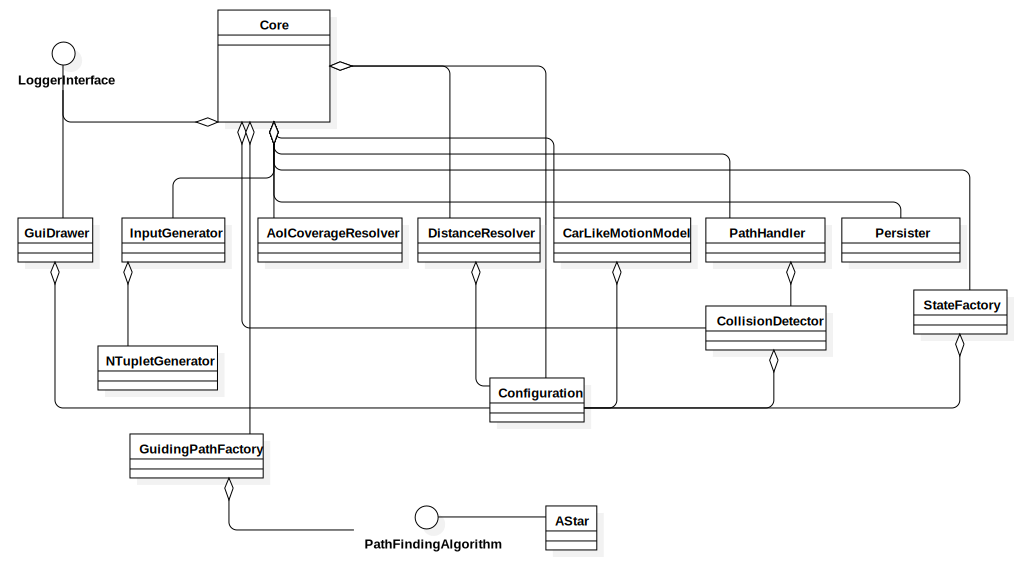
\includegraphics[scale=0.4]{obrazky/umlSchema}

Core class holds core of whole Application and has all other classes
as dependencies, as is shown in image above. 

State factory creates State classes according to Factory pattern.
State class represents state in RRT-Path algorithm. State has coordinates
and rotations for all UAVs.

Persister persists found path to JSON using Json Spirit library.

PathHandler serves as utils class for manipulations with path (vector
of State classes).

CarLikeMotionModel holds motion model algorithm.
\begin{thebibliography}{1}
\bibitem[1]{Dubins-thesis}Petr Váňa,\emph{ Path Planning for Non-holonomic
Vehicle in Surveillance Missions} {[}online{]}. {[}cit. 2015-12-29{]}.
Dostupný z WWW: \url{https://dspace.cvut.cz/bitstream/handle/10467/61814/F3-DP-2015-Vana-Petr-thesis.pdf}

\end{thebibliography}
\cleardoublepage{}
\end{document}
